\RequirePackage{amssymb}
\documentclass[a4paper,UKenglish,cleveref,autoref,thm-restate]{tgdk-v2021}

% Pre-submission draft: suppresses provisional DOI, volume, and issue metadata.
\hideTGDK

\bibliographystyle{plainurl}

\usepackage{booktabs}
\usepackage{tabularx}
\usepackage{array}
\usepackage{float}
\usepackage{graphicx}
\usepackage{tikz}
\usetikzlibrary{arrows.meta,positioning,fit,calc,shapes.geometric}

\title{The Fidelity--Safety Gap in Neural Repair of Wikidata Constraint Violations}
\titlerunning{The Fidelity--Safety Gap in Neural Repair of Wikidata Constraint Violations}

\author{Miguel V\'azquez}{Vienna University of Economics and Business (WU Wien), Vienna, Austria}{miguel.vazquez@wu.ac.at}{https://orcid.org/0009-0002-9067-959X}{}
\author{Axel Polleres}{Vienna University of Economics and Business (WU Wien), Vienna, Austria}{axel.polleres@wu.ac.at}{https://orcid.org/0000-0001-5670-1146}{}

\authorrunning{M. V\'azquez and A. Polleres}
\Copyright{Miguel V\'azquez and Axel Polleres}

\ccsdesc{Information systems~Data cleaning}
\ccsdesc{Information systems~Resource Description Framework (RDF)}
\ccsdesc{Computing methodologies~Neural networks}
\ccsdesc{Theory of computation~Logic and verification}

\keywords{Wikidata, Knowledge Graph Repair, Property Constraints, Graph Neural Networks, Neuro-Symbolic Learning, Data Quality, Repair Evaluation}

\supplementdetails[subcategory={Source Code and Configurations; MIT},linktext={release v1.0.0}]{Software}{https://github.com/miguelvc6/fidelity-safety-gap/releases/tag/v1.0.0}
\supplementdetails[subcategory={Benchmark Inputs and Evaluation Results; CC BY 4.0},linktext={Zenodo 22013512}]{Dataset}{https://doi.org/10.5281/zenodo.22013512}
\supplementdetails[subcategory={Trained Checkpoints; CC BY 4.0},linktext={Zenodo 22013512}]{Model}{https://doi.org/10.5281/zenodo.22013512}
\supplementdetails[subcategory={Supplementary Results; CC BY 4.0},linktext={Zenodo 22013512}]{Text}{https://doi.org/10.5281/zenodo.22013512}
\funding{This research was funded in whole or in part by the Austrian Science Fund (FWF)\\ 10.55776/COE12.}

% EditorialOffice macros (do not touch as author)
\Volume{1}
\Issue{1}
\Article{42}
\DateSubmission{Date of submission}
\DateAcceptance{Date of acceptance}
\DatePublished{Date of publishing}
\SectionAreaEditor{TGDK section area editor}

\newcommand{\kg}{KG}
\newcommand{\kgs}{KGs}
\newcommand{\locsat}{\mathrm{LocalSat}}
\newcommand{\sir}{\mathrm{SIR}}
\newcommand{\srr}{\mathrm{SRR}}
\newcommand{\bppf}{\mathrm{BPPF}}
\newcommand{\Gpre}{G_i^{\mathrm{pre}}}
\newcommand{\Ghist}{G_i^{\mathrm{hist}}}
\newcommand{\Gpred}{G_i^{\mathrm{pred}}}
\newcommand{\histedit}{\Delta^{\mathrm{H}}}
\newcommand{\prededit}{\Delta^{\mathrm{P}}}
\newcommand{\witnessctx}{\mathcal{W}}
\newcommand{\maskedprededit}[2]{\Delta^{\mathrm{P}}_{#1,#2}}
\begin{document}

\maketitle

\begin{abstract}
Collaborative knowledge graphs such as Wikidata use property constraints to flag candidate errors for curation. Detecting a violation, however, does not determine its repair: multiple edits may satisfy the same constraint while differing in information content, curator agreement, and collateral effects. Recorded historical edits allow models to learn curation conventions and statistical patterns, but learned models provide no formal guarantee that a predicted edit will satisfy the associated constraint definition or avoid collateral violations. We study this gap between validation and learned repair imitation.

We represent each historical correction case as a violation-centred graph and augment a graph neural network (GNN) with dedicated nodes representing locally selected constraint definitions. These \emph{neural constraint factors} learn to predict constraint satisfaction and exchange messages with nodes in their local scope through explicit message channels. These channels can be selectively suppressed at inference time to inspect how constraint information affects repair predictions.

Using a corpus of 955,405 Wikidata repair instances, we evaluate all reported systems on a held-out test split of 143,316 instances. The factor GNN reaches 0.6788 F1 for agreement with recorded historical statement edits, compared with 0.5471 for a vanilla GNN. Suppressing factor messages drops F1 to 0.2803 (a decrease of 0.3985) and changes 58.6\% of predictions.

When we re-evaluate predicted edits with local symbolic validators, a different trade-off emerges. We train \textsc{Candidate-DP} to select among candidate edits by prioritising fixing the primary constraint definition while penalising collateral violations. While it raises the primary fix rate from 62.78\% to 77.07\% and slightly reduces collateral regressions (0.48\% to 0.39\%), it substantially harms historical fidelity (F1 falls from 0.6788 to 0.4370). More starkly, a reranker trained solely to maximise constraint satisfaction (\textsc{Candidate-SR}) degenerates into a near-universal deletion strategy, removing the base statement in 97.41\% of cases. This learned satisfaction-by-deletion shortcut demonstrates that constraint satisfaction alone can reward removing evidence rather than useful correction.

By making constraint pathways explicit and separating imitation from symbolic validation, this work provides a principled foundation for inspectable, preservation-aware automated KG curation.
\end{abstract}

\section{Introduction}
\label{sec:introduction}

Collaborative knowledge graphs (KGs) such as Wikidata evolve through continuous community contributions and inevitably accumulate incomplete, inconsistent, or otherwise questionable statements \cite{hogan2021knowledge,vrandecic2014wikidata,polleres2023evolution,shenoy2022quality}. Wikidata supports quality control through \emph{property constraints}, which describe how properties are normally expected to be used. Unlike hard database constraints, they flag violations for review rather than rejecting non-conforming edits \cite{ferranti2024formalizing,wikidataPropertyConstraintsPortal,wikibaseQualityConstraints}. Detecting a violation therefore identifies a problem, but does not determine how it should be repaired.

A historical violation record identifies a focal statement, which we call the \emph{base statement}, and may also identify or imply additional witness statements or qualifiers that supply context \cite{bertossi2022database,ahmetaj2022repairing,ahmetaj2025logic,ferranti2025repairs}. Candidate edits include adding missing information, replacing conflicting values, or deleting an implicated statement. Historical edits provide supervision for choosing among such alternatives, and previous work has used them to train statistical and neural correction systems \cite{pellissier2019learning,pellissier2021neural}. More recently, graph neural networks (GNNs) have shown that local graph structure is a strong signal for reproducing recorded Wikidata edits \cite{vazquez2026structure}.

However, reproducing historical edits and producing a useful repair are not equivalent objectives. Agreement with a curator's recorded edit does not guarantee that the primary constraint definition becomes satisfied or that other local constraint definitions remain satisfied. Conversely, constraint satisfaction alone does not determine whether an edit is desirable: deleting the base statement may remove the evidence for a violation while also discarding useful information, while a constraint-compliant replacement may still be factually incorrect. Existing learned repair approaches and formal validation therefore provide complementary but incomplete views of repair quality. It remains unclear how historical fidelity relates to post-edit constraint behaviour, whether explicitly providing constraint information to a learned model can help, and what happens when constraint satisfaction directly influences repair decisions. We refer to this tension as the \emph{fidelity--safety gap}. % Throughout the paper, \emph{repair safety} is an umbrella term for bounded post-edit constraint behaviour and base-statement preservation; it is not a guarantee of global Wikidata constraint satisfaction.

We study this gap using a GNN over violation-centred subgraphs derived from historical Wikidata correction records \cite{vazquez2026structure}. We augment each subgraph with nodes that encode property-constraint definitions associated with properties represented in the subgraph. For each such definition, the GNN includes a dedicated \emph{neural constraint factor} that reads the representations of the relevant local nodes and passes learned constraint information back to them. These factors learn from labels produced by symbolic validators. % The validators themselves do not execute edits during neural inference; instead, they provide supervision during training and evaluation. This separation lets us examine whether explicit constraint information improves prediction of recorded historical edits while also measuring what the resulting predicted edits do to the local constraint state.

\paragraph*{Research questions.}
We organise the study around three questions:
\begin{enumerate}
    \item \textbf{Predictive fidelity (RQ1):} Does explicitly representing locally selected constraint definitions improve agreement with recorded historical edits relative to standard neural and heuristic baselines?
    \item \textbf{Constraint use (RQ2):} Do neural constraint factors encode information aligned with symbolic validation, and do their messages materially influence edit decisions?
    \item \textbf{Fidelity--safety divergence (RQ3):} How does historical fidelity relate to post-edit constraint outcomes, and where do these objectives diverge?
\end{enumerate}

We evaluate repair quality not only by agreement with recorded historical edits, but also by whether the primary constraint definition is fixed, whether secondary local definitions improve or regress, how many additions and deletions the predicted edit makes, and whether the base statement is preserved. On a corpus of 955,405 Wikidata repair instances, with 143,316 held out for testing, the GNN with neural constraint factors reaches 0.6788 F1 for historical agreement, compared with 0.5471 for a vanilla GNN. Removing factor messages at inference substantially changes predictions and sharply reduces fidelity, showing that the trained model actively uses the constraint pathway.

To probe the divergence directly, we also compare complete candidate edits under objectives that increasingly prioritise their symbolic consequences. Incorporating constraint-based penalties substantially improves primary-constraint resolution, but at the cost of historical fidelity and base-statement preservation. More strikingly, a diagnostic reranker trained solely for local constraint satisfaction and ignoring historical fidelity converges toward an almost universal deletion strategy, removing the base statement in 97.41\% of test cases. This satisfaction-by-deletion behaviour demonstrates that constraint satisfaction alone is insufficient as a repair objective.

The central finding is a mismatch between historical imitation and constraint validation: better agreement with recorded historical edits does not guarantee better post-edit constraint behaviour, while optimising constraint satisfaction can reward destructive deletion. Learned KG repair should therefore treat historical fidelity, local constraint satisfaction, and information preservation as distinct objectives rather than interchangeable proxies for repair quality.

\paragraph*{Contributions.}
This paper makes four main contributions:
\begin{itemize}
    \item We introduce \textbf{neural constraint factors (Section~\ref{sec:neural-constraint-factors})}, an explicit and inspectable representation of locally selected, validator-supported Wikidata property-constraint definitions within a GNN repair model.
    \item We develop a \textbf{multi-dimensional evaluation (Section~\ref{sec:evaluation})} that distinguishes agreement with recorded historical edits from whether the primary constraint definition is fixed, how secondary definitions change, and whether the base statement identified by the violation record is preserved rather than removed.
    \item By showing that factor states predict symbolic validator outcomes, and by removing factor messages at inference time, we show that the learned model \textbf{uses the explicit constraint pathway} in making repair decisions.
    \item We empirically characterise the \textbf{fidelity--safety gap (Section~\ref{sec:experiments},~\ref{sec:results} and~\ref{sec:discussion})}, showing that improved constraint satisfaction can come at the cost of historical fidelity and that satisfaction-only optimisation admits a deletion shortcut.
\end{itemize}

\section{Related Work}
\label{sec:related-work}

\subsection{Constraint validation and symbolic repair}

Constraint languages such as SHACL and ShEx provide mechanisms for validating RDF graphs \cite{w3cSHACL2017,shex2019spec}. Wikidata's property constraints have likewise been formalised through SHACL and SPARQL \cite{ferranti2024formalizing}, logical frameworks \cite{martin2020mars,marx2017logic}, and Wikibase-oriented shape languages such as WShEx \cite{labra2022wshex}. These approaches establish whether data conforms to specified constraints; our work instead focuses on selecting and evaluating repairs once a violation has been identified.

Symbolic repair additionally considers how validity can be restored. Database repair provides foundations for repair semantics and minimal change \cite{bertossi2022database}, while SHACL repair has addressed explanations and preferred repairs, including through answer-set programming \cite{ahmetaj2021explanations,ahmetaj2022repairing,ahmetaj2025logic}. Related work on axiom weakening explicitly considers information preservation \cite{troquard2018weakening}. For Wikidata specifically, Ferranti et al.~\cite{ferranti2025repairs} formalise constraint-violation repairs and characterise the repair patterns observed in curator edits. We complement these approaches by learning repair choices from historical edits while independently revalidating their post-edit constraint consequences.

\subsection{Learning-based KG repair}

Historical Wikidata edits have been used to train statistical and neural correction systems \cite{pellissier2019learning,pellissier2021neural}. More broadly, learning-based KG quality methods include anomaly detection, plausibility scoring, link prediction, and refinement \cite{paulheim2017refinement,subagdja2024refining,zhang2022caged}; however, our setting requires predicting a concrete edit whose consequences can subsequently be validated.

Our closest predecessor is V\'azquez et al.~\cite{vazquez2026structure}, who encode historical Wikidata correction cases as local multi-relational graphs and show that GNNs can exploit graph structure to reproduce curator edits. We retain this edit-prediction task but extend it in two directions: locally selected property-constraint definitions become explicit components of the learned model, and predicted edits are independently evaluated through symbolic validation. % This allows us to study whether historical fidelity and post-edit constraint behaviour agree rather than treating reproduction of the recorded edit as the sole notion of success.

\subsection{Neuro-symbolic constraint integration}

Neuro-symbolic methods incorporate structured knowledge into neural learning through logical or differentiable objectives \cite{xu2018semantic,fischer2019dl2,yang2022clste}, constrained structured prediction \cite{jiang2022coresp}, and neural message passing over factor graphs \cite{zhang2023fgnn,garciasatorras2021nebp}. Our architecture is closest to the latter: constraints act as local computational units that exchange information with the graph. Unlike generic learned factors, however, each of our neural constraint factors corresponds to a concrete Wikidata constraint definition selected within a repair instance and is supervised by a separate symbolic validator. % Keeping symbolic validation outside the neural forward pass allows us to evaluate two questions separately: whether the model learns and uses constraint-related information, and whether its predicted edits actually improve the resulting constraint state.

\section{Background: Wikidata Constraints and Repairs}
\label{sec:background}

Wikidata contains two main kinds of entities: \emph{items} and \emph{properties}. Items represent real-world objects or abstract concepts, such as people, places, or events, while properties describe relations or attributes of items, such as \emph{country of citizenship} or \emph{date of birth}. Wikidata represents statements as subject--predicate--object triples \(\tau=(s,p,o)\), where \(s\) is an item, \(p\) is a property, and \(o\) is an item or literal (data values such as strings, numbers, coordinates, or dates). Statements can also be expanded, annotated, or contextualized with additional values, as well as optional qualifiers, references, and ranks \cite{wikidataDataModel,vrandecic2014wikidata}. Wikidata can therefore be viewed as a directed, edge-labelled graph: items and literals form the nodes, while properties define the labelled edges connecting them. Throughout this paper, \emph{statement} refers to this triple abstraction; ranks, qualifiers, and references are outside the repair language.

A Wikidata \emph{property constraint} is metadata attached to a property and encoded as a statement with property \texttt{P2302}. Its value identifies the \emph{constraint type}, that is, the kind of rule being applied, such as single-value, value-type, inverse, or conflicts-with. The qualifiers of the \texttt{P2302} statement provide the \emph{constraint parameters}; for example, a value-type constraint may specify the required class of the object \(o\) \cite{ferranti2024formalizing,ferranti2025repairs, wikidataPropertyConstraintsPortal,wikibaseQualityConstraints}. We use \emph{constraint definition} for a concrete constraint on a particular property, including its type and parameters.

A historical violation record associates a constraint definition with a \emph{base statement}: the statement whose property is constrained. Some recorded violations also depend on additional local evidence: a conflicts-with violation requires a conflicting statement, while distinct-values or single-value violations require another statement sharing a value or property. Inverse or item-requires-statement violations may instead depend on missing expected evidence. Following Ferranti et al.~\cite{ferranti2025repairs}, we use \emph{witness pattern} for the symbolic pattern of present or missing statements and constraint metadata that characterises a violation, and \emph{witness context} for the set of additional local statements, beyond the base statement, used to evaluate the recorded violation. This set may be empty when the violation does not require additional present statements. A \emph{repair action} is an edit proposed to address a recorded violation; whether it is a successful repair is determined by post-edit symbolic validation.

For a constraint definition \(c\) whose type has an implemented validator, its local evaluation within a repair instance on a bounded symbolic state \(G\) returns \emph{satisfied}, \emph{violated}, or \emph{unknown}. It returns \emph{unknown} when the required constraint parameters or local evidence are unavailable. We call this evaluation \emph{checkable} in the first two cases and \emph{uncheckable} in the third. Thus, uncheckability denotes insufficient evidence for a Boolean decision rather than a violation; definitions without an implemented validator receive no validation outcome. % Checkability is state-dependent and may change after an edit.

Although Wikidata itself does not enforce a strict description-logic separation, the A-box/T-box abstraction is useful for delimiting the repair space. We distinguish A-box repairs, which modify statements or qualifiers, from T-box repairs, which modify constraint definitions . We restrict this study to A-box edits learned from historical correction records. % The full Wikidata repair space includes qualifiers, ranks, references, and T-box changes; these matter for complete Wikidata repair but are outside the six-slot statement prediction task evaluated here.

\section{Task and Problem Formulation}
\label{sec:task}

\subsection{Repair instances and edits}
\label{sec:task:instance}
A repair instance is a historical correction record associated with a recorded property-constraint violation, together with its bounded local evidence and observed edit:
\[
i=(\tau_i,\witnessctx_i,\mathcal{A}_i,\mathcal{C}_i,\histedit_i),
\qquad
\tau_i=(s_i,p_i,o_i).
\]
Here, \(\tau_i\) is the base statement identified by the historical violation record, \(\witnessctx_i\) is the witness context, \(\mathcal{A}_i\) is the one-hop outgoing A-box neighbourhood, \(\mathcal{C}_i\) is the set of concrete constraint definitions selected for the instance from properties represented in its local neighbourhood, and \(\histedit_i\) is the recorded historical edit. The definition \(c_i^\star\in\mathcal{C}_i\) is the \emph{primary constraint definition} associated with the historical violation record; the remaining elements are \emph{secondary constraint definitions}. Each concrete definition appears at most once in \(\mathcal{C}_i\), even when its constrained property occurs in multiple local statements.

\label{sec:task:action}
An edit contains at most one fully specified statement addition and one fully specified statement deletion:
\[
\Delta=(\tau^+,\tau^-).
\]
Each component is either a statement triple or absent: when present, \(\tau_i^+=(s^+,p^+,o^+)\) denotes the added statement and \(\tau^-=(s^-,p^-,o^-)\) denotes the deleted statement; otherwise the corresponding component is \(\bot\). A replacement therefore consists of both a deletion and an addition. Both the historical edit \(\histedit_i\) and a model's predicted edit \(\prededit_i\) use this representation.

\subsection{Bounded symbolic edit states}
\label{subsec:symbolic-states}

For each repair instance, the symbolic evaluator reconstructs a bounded pre-edit state from the statement triples supplied in the instance:
\[
G_i^{\mathrm{pre}}=\{\tau_i\}\cup\mathcal{W}_i\cup\mathcal{A}_i.
\]
The historical and predicted edits are applied independently to this common state, yielding
\[
G_i^{\mathrm{hist}}=\operatorname{apply}(G_i^{\mathrm{pre}},\histedit_i),
\qquad
G_i^{\mathrm{pred}}=\operatorname{apply}(G_i^{\mathrm{pre}},\prededit_i).
\]
% For an edit \(\Delta=(\tau^+,\tau^-)\), \(\operatorname{apply}(G,\Delta)\) first removes \(\tau^-\) when \(\tau^-\neq\bot\) and then inserts \(\tau^+\) when \(\tau^+\neq\bot\). Because evaluation is restricted to the bounded local instance, an operation modifies the symbolic state only when its subject and property lie within the represented local scope; otherwise it remains part of the predicted edit for historical-fidelity and edit-size metrics but has no effect on local constraint validation.

The states \(G_i^{\mathrm{pre}}\), \(G_i^{\mathrm{hist}}\), and \(G_i^{\mathrm{pred}}\) are sets of statement triples used for symbolic supervision and evaluation. They are distinct from the neural input representation introduced in \cref{sec:neural-constraint-factors}.

\subsection{Local validator semantics}
\label{subsec:validator-semantics}

The validators operate on the bounded symbolic states defined in \cref{subsec:symbolic-states}. They neither query the complete Wikidata graph nor use information outside the bounded local evidence. In particular, typing constraints are evaluated using only the available \texttt{P31} (\emph{instance of}) and \texttt{P279} (\emph{subclass of}) statements; the global transitive class hierarchy is not traversed.

To specify the validators uniformly across constraint types, we introduce three shared components: access to locally represented property values, conditions determining whether the required local evidence is available, and the anchor at which a constraint definition is evaluated. Together with the definition's parameters, these components determine whether its local evaluation is \emph{checkable} on a state \(G\) and, when checkable, whether it is \emph{satisfied}. We define this common notation below before giving the type-specific validator semantics in Table~\ref{tab:validator-semantics}.

For any property \(p\) and state \(G\), define
\[
p^G(s)=\{o\mid (s,p,o)\in G\},
\]
the set of locally represented values of \(p\) for entity \(s\). In particular, let \(p_c\) denote the property constrained by definition \(c\); then \(p_c^G(s)\) denotes the locally represented values of the property constrained by \(c\). We call an entity--property pair \((s,p)\) \emph{locally decidable} in \(G\), written \(\operatorname{dec}_G(s,p)\), when \(s\) is represented, \(p\) lies within the instance's local predicate closure, and every edit operation targeting \((s,p)\) can be applied to the local state. For such a pair, the evaluator interprets \(p^G(s)=\varnothing\) as the local absence of values for \(p\) within the bounded local state. This closed-world assumption applies only to the bounded instance and does not imply that Wikidata itself is complete.

Checkability reflects the same evidence boundary. As described in \cref{subsec:symbolic-states}, an operation outside the represented subject or predicate scope does not modify \(G\). If a validator depends on the corresponding unresolved entity--property pair, its outcome is therefore \emph{unknown}. The typing-related validators are additionally conservative: when their constrained-property trigger remains present but the required local typing evidence is absent, they return \emph{unknown} rather than treating missing type information as a violation.

After resolving the Wikidata item and property IDs contained in each constraint definition, the evaluator constructs the constraint parameter sets
\begin{itemize}
    \item \(\mathrm{Req}_c\) from \texttt{P2306} (\emph{property}),
    \item \(\mathrm{Items}_c\) from \texttt{P2305} (\emph{item of property constraint}),
    \item \(\mathrm{Class}_c\) from \texttt{P2308} (\emph{class}),
    \item \(\mathrm{Conf}_c\) from the conflicting properties of the conflicts-with definition,
    \item \(\mathrm{Inv}_c\) from \texttt{P1696} (\emph{inverse property}), defaulting to \(p_c\), and
    \item \(\mathrm{Rel}_c\) from \texttt{P2309} (\emph{relation}), defaulting to \texttt{P31} (\emph{instance of}) and \texttt{P279} (\emph{subclass of}).
\end{itemize}

Constraint parameters are extracted from the corresponding Wikidata qualifiers and included in these sets only when their values can be mapped to a Wikidata item or property ID. If a validator in Table~\ref{tab:validator-semantics} requires a non-empty parameter set but no such parameter is available, the local evaluation of the constraint definition is treated as uncheckable.

\begin{table}[p]
\caption{Type-specific semantics of the bounded local validators. The satisfaction condition is evaluated only after the checkability condition holds.}
\label{tab:validator-semantics}
\centering
\fontsize{6.5}{7}\selectfont
\renewcommand{\arraystretch}{1.00}
\setlength{\jot}{0pt}
\setlength{\tabcolsep}{3pt}
\resizebox{\textwidth}{!}{%
\begin{tabularx}{1.14\textwidth}{@{}
  >{\raggedright\arraybackslash\hsize=.65\hsize}X
  >{\raggedright\arraybackslash\hsize=.90\hsize}X
  >{\raggedright\arraybackslash\hsize=1.25\hsize}X
  >{\raggedright\arraybackslash\hsize=1.25\hsize}X
  >{\raggedright\arraybackslash\hsize=.95\hsize}X@{}}
\toprule
\textbf{Constraint type} &
\textbf{Anchor and parameters} &
\textbf{Checkable when} &
\textbf{Satisfied when} &
\textbf{Bounded-evidence limitation} \\
\midrule

Conflicts-with
&
Subject \(s_i\);
\(p_c,\mathrm{Conf}_c,\)\newline
\(\mathrm{Items}_c\)
&
\(
\begin{aligned}
&\mathrm{Conf}_c\neq\varnothing
\land \operatorname{dec}_G(s_i,p_c)
\\[-1pt]
&{}\land\forall p\in\mathrm{Conf}_c:\,
\operatorname{dec}_G(s_i,p)
\end{aligned}
\)
&
\(
\begin{aligned}
&p_c^G(s_i)=\varnothing
\\[-1pt]
&{}\lor\forall p\in\mathrm{Conf}_c:\,
\\[-1pt]
&\quad\bigl[(\mathrm{Items}_c=\varnothing
\\[-1pt]
&\qquad{}\land p^G(s_i)=\varnothing)
\\[-1pt]
&\quad{}\lor
  (\mathrm{Items}_c\neq\varnothing
   \land p^G(s_i)
\\[-1pt]
&\qquad\quad{}
   \cap\mathrm{Items}_c=\varnothing)
\bigr]
\end{aligned}
\)
&
-- \\
\addlinespace[7pt]

Distinct-values
&
Base \(\tau_i\);
recorded witness \(\tau_i^{\mathrm{w}}=(s_i^{\mathrm{w}},p_i^{\mathrm{w}},o_i^{\mathrm{w}})\)
&
\(
\begin{aligned}
&\operatorname{dec}_G(s_i,p_c)
\\[-1pt]
&{}\land\bigl[\tau_i\in G\Rightarrow
\\[-1pt]
&\quad(\text{witness complete}
\\[-1pt]
&\qquad{}\land p_i^{\mathrm{w}}=p_c)\bigr]
\end{aligned}
\)
&
\(
\begin{aligned}
\neg\bigl(&\tau_i\in G\land p_i^{\mathrm{w}}=p_c
\\[-1pt]
&{}\land o_i^{\mathrm{w}}=o_i\land s_i^{\mathrm{w}}\neq s_i\bigr)
\end{aligned}
\)
&
Compares only locally represented statements. \\
\addlinespace[7pt]

Inverse
&
Base \(\tau_i\);
\(p_c,\mathrm{Inv}_c\)
&
\(
\begin{aligned}
&p_i=p_c
\land \operatorname{dec}_G(s_i,p_c)
\\[-1pt]
&{}\land
\bigl[
\tau_i\in G
\Rightarrow
  (\mathrm{Inv}_c\neq\varnothing
\\[-1pt]
&\qquad{}\land
  \forall p\in\mathrm{Inv}_c:\,
\\[-1pt]
&\qquad\quad
  \operatorname{dec}_G(o_i,p)
)
\bigr]
\end{aligned}
\)
&
\(
\begin{aligned}
&\tau_i\notin G
\\[-1pt]
&{}\lor\exists p\in\mathrm{Inv}_c:\,
 (o_i,p,s_i)\in G
\end{aligned}
\)
&
Compares only locally represented statements. \\
\addlinespace[7pt]

Symmetric
&
Base \(\tau_i\);
\(p_c\)
&
\(
\begin{aligned}
&p_i=p_c
\land \operatorname{dec}_G(s_i,p_c)
\\[-1pt]
&{}\land\bigl[\tau_i\in G\Rightarrow
\operatorname{dec}_G(o_i,p_c)
\bigr]
\end{aligned}
\)
&
\(
\tau_i\notin G\lor (o_i,p_c,s_i)\in G
\)
&
-- \\
\addlinespace[7pt]

Item-requires-\newline statement
&
Subject \(s_i\);
\(p_c,\mathrm{Req}_c,\)\newline
\(\mathrm{Items}_c\)
&
\(
\begin{aligned}
&\mathrm{Req}_c\neq\varnothing
\land \operatorname{dec}_G(s_i,p_c)
\\[-1pt]
&{}\land\bigl[p_c^G(s_i)\neq\varnothing
\Rightarrow
\\[-1pt]
&\qquad\forall p\in\mathrm{Req}_c:\,
\\[-1pt]
&\qquad\quad\operatorname{dec}_G(s_i,p)
\bigr]
\end{aligned}
\)
&
\(
\begin{aligned}
&p_c^G(s_i)=\varnothing
\\[-1pt]
&{}\lor\forall p\in\mathrm{Req}_c:\,
\\[-1pt]
&\quad\bigl[(\mathrm{Items}_c=\varnothing
\\[-1pt]
&\qquad{}\land p^G(s_i)\neq\varnothing)
\\[-1pt]
&\quad{}\lor
  (\mathrm{Items}_c\neq\varnothing
   \land p^G(s_i)
\\[-1pt]
&\qquad\quad{}
   \cap\mathrm{Items}_c\neq\varnothing)
\bigr]
\end{aligned}
\)
&
-- \\
\addlinespace[7pt]

Value-requires-\newline statement
&
Base value \(o_i\);
\(p_c,\mathrm{Req}_c,\)\newline
\(\mathrm{Items}_c\)
&
\(
\begin{aligned}
&p_i=p_c
\land \operatorname{dec}_G(s_i,p_c)
\\[-1pt]
&{}\land\bigl[\tau_i\in G\Rightarrow
  (\mathrm{Req}_c\neq\varnothing
\\[-1pt]
&\qquad{}\land
  \forall p\in\mathrm{Req}_c:\,
\\[-1pt]
&\qquad\quad
  \operatorname{dec}_G(o_i,p)
)
\bigr]
\end{aligned}
\)
&
\(
\begin{aligned}
&\tau_i\notin G
\\[-1pt]
&{}\lor\forall p\in\mathrm{Req}_c:\,
\\[-1pt]
&\quad\bigl[(\mathrm{Items}_c=\varnothing
\\[-1pt]
&\qquad{}\land p^G(o_i)\neq\varnothing)
\\[-1pt]
&\quad{}\lor
  (\mathrm{Items}_c\neq\varnothing
   \land p^G(o_i)
\\[-1pt]
&\qquad\quad{}
   \cap\mathrm{Items}_c\neq\varnothing)
\bigr]
\end{aligned}
\)
&
Only the recorded base value \(o_i\) is inspected. \\
\addlinespace[7pt]

One-of
&
Subject \(s_i\);
\(p_c,\mathrm{Items}_c\)
&
\(
\mathrm{Items}_c\neq\varnothing
\land\operatorname{dec}_G(s_i,p_c)
\)
&
\(
p_c^G(s_i)\subseteq\mathrm{Items}_c
\)
&
-- \\
\addlinespace[7pt]

Single-value
&
Subject \(s_i\);
\(p_c\)
&
\(
\operatorname{dec}_G(s_i,p_c)
\)
&
\(
\lvert p_c^G(s_i)\rvert\leq 1
\)
&
-- \\
\addlinespace[7pt]

Subject type
&
Subject \(s_i\);
\(p_c,\mathrm{Class}_c,\)\newline
\(\mathrm{Rel}_c\)
&
\(
\begin{aligned}
&\mathrm{Class}_c\neq\varnothing
\land \operatorname{dec}_G(s_i,p_c)
\\[-1pt]
&{}\land\bigl[p_c^G(s_i)\neq\varnothing
\Rightarrow
\\[-1pt]
&\quad(
  \mathrm{Rel}_c\neq\varnothing
  \land
  \forall p\in\mathrm{Rel}_c:\,
\\[-1pt]
&\qquad\quad
  \operatorname{dec}_G(s_i,p)
\\[-1pt]
&\qquad{}\land
  \bigcup_{p\in\mathrm{Rel}_c}p^G(s_i)
  \neq\varnothing
)
\bigr]
\end{aligned}
\)
&
\(
\begin{aligned}
&p_c^G(s_i)=\varnothing
\\[-1pt]
&{}\lor\left(
  \bigcup_{p\in\mathrm{Rel}_c}p^G(s_i)
\right)
\\[-1pt]
&\qquad{}\cap\mathrm{Class}_c
\neq\varnothing
\end{aligned}
\)
&
Uses direct local class matches only; no global transitive class hierarchy is followed. \\
\addlinespace[7pt]

Value-type
&
Focal value \(o_i\);
\(p_c,\mathrm{Class}_c,\)\newline
\(\mathrm{Rel}_c\)
&
\(
\begin{aligned}
&o_i\text{ resolved}
\land \mathrm{Class}_c\neq\varnothing
\\[-1pt]
&{}\land \operatorname{dec}_G(s_i,p_c)
\\[-1pt]
&{}\land\bigl[p_c^G(s_i)\neq\varnothing
\Rightarrow
\\[-1pt]
&\quad(
  \mathrm{Rel}_c\neq\varnothing
  \land
  \forall p\in\mathrm{Rel}_c:\,
\\[-1pt]
&\qquad\quad
  \operatorname{dec}_G(o_i,p)
\\[-1pt]
&\qquad{}\land
  \bigcup_{p\in\mathrm{Rel}_c}p^G(o_i)
  \neq\varnothing
)
\bigr]
\end{aligned}
\)
&
\(
\begin{aligned}
&p_c^G(s_i)=\varnothing
\\[-1pt]
&{}\lor\left(
  \bigcup_{p\in\mathrm{Rel}_c}p^G(o_i)
\right)
\\[-1pt]
&\qquad{}\cap\mathrm{Class}_c
\neq\varnothing
\end{aligned}
\)
&
The class test remains anchored to \(o_i\); no global transitive class hierarchy is followed. \\

\bottomrule
\end{tabularx}%
}
\end{table}

% A consequence of these bounded, anchor-specific semantics is that deletion can affect local constraint evaluations in qualitatively different ways. For distinct-values, inverse, symmetric, and value-requires-statement, the satisfaction condition explicitly becomes true when the exact base statement \(\tau_i\) is absent, provided the remaining checkability requirements hold. This behaviour is not shared uniformly by the other constraint types. Because the same statement may occupy different roles in different constraint definitions, deleting \(\tau_i\) may instead remove a constrained-property trigger, conflicting evidence, required evidence, typing evidence, or only one value from a locally evaluated property set. For example, single-value is satisfied once the local cardinality falls to at most one, whereas deleting one one-of value does not help if another disallowed value remains. For subject type and value-type, removing the last locally represented typing evidence while leaving the constrained-property trigger present makes the local evaluation uncheckable rather than violated. These differences are important when interpreting post-edit satisfaction: an increase can result from a targeted correction, from removal of relevant evidence, or from a change in what remains locally checkable.

Section~\ref{sec:evaluation} evaluates each predicted edit both against the recorded historical edit and by revalidating its consequences on the bounded post-edit state.

\section{Neural Constraint Factors}
\label{sec:neural-constraint-factors}

Predicting an edit requires combining the local graph structure with information about the property constraints that apply to it. 

A standard GNN encoder can propagate information through the local statements and constraint definitions represented in the input, but it does not explicitly specify which nodes play distinct semantic roles for a particular constraint or how their representations should interact. We therefore introduce \emph{neural constraint factors}: learned computational units that represent individual constraint definitions, read the nodes in their local scopes, and return constraint-conditioned messages to those nodes.

The resulting architecture alternates between a graph-encoder update over the input graph and a factor update over the represented constraint definitions. The graph encoder is a modular component; the experiments instantiate it with GINE \cite{xu2019gin,hu2020gine}. The symbolic validators are not executed inside this neural forward pass. They provide auxiliary satisfaction labels during training and are used independently for post-edit evaluation. We call the complete architecture the \emph{Direct--Factor GNN}.

\subsection{Factorised model input}
\label{subsec:factor-graph}

This subsection describes how each repair instance is represented as input to the neural models. The representation comprises a graph processed by the graph encoder and role-specific scopes used by the neural constraint factors.

For each constraint definition \(c\in\mathcal{C}_i\), let \(t_c\) denote its constraint type. Only definitions for which symbolic validators are implemented are represented by neural factors. We denote this subset by
\[
\mathcal{C}_i^{\mathrm{fac}}=\{c\in\mathcal{C}_i\mid\text{a symbolic validator is implemented for }t_c\}.
\]
For each \(c\in\mathcal{C}_i^{\mathrm{fac}}\), the model creates exactly one factor node \(f_c\).

\paragraph*{Graph-encoder representation.} The graph-encoder input comprises a node set \(\mathcal{Z}_i\) and a directed multiset of encoder edges \(\mathcal{E}_i^{\mathrm{enc}}\), constructed from the local statements and constraint definitions included in repair instance \(i\).

Each statement \(\tau=(s,p,o)\) is represented by three state-bearing nodes: term nodes for its subject \(s\) and object \(o\), and a fresh predicate-occurrence node \(p_\tau\) representing property \(p\) in that particular statement. Distinct statements using the same property therefore have distinct predicate-occurrence nodes.

The encoder edge itself connects the subject to the object, \(e_\tau:s\xrightarrow{p_\tau}o\). Here, the hidden state of \(p_\tau\) is used to construct the edge feature during graph-encoder message passing. We write the edge record as \(e_\tau=(s,p_\tau,o)\). Using a separate node for each predicate occurrence allows different statements using the same property to maintain distinct hidden states, while still sharing the categorical representation of the underlying property.

Constraint parameters use the same representation. For each \(c\in\mathcal{C}_i^{\mathrm{fac}}\), let \(\Theta_c\) denote its set of parameter pairs. A parameter \(\theta=(q,a)\in\Theta_c\) consists of a parameter property \(q\) and its value \(a\). It contributes the factor node \(f_c\), the parameter-value node \(a\), and a fresh predicate-occurrence node \(q_\theta\) representing \(q\) in that parameter. The corresponding encoder edge is \(e_{c,\theta}:f_c\xrightarrow{q_\theta}a\), equivalently \(e_{c,\theta}=(f_c,q_\theta,a)\). The edge multiset \(\mathcal{E}_i^{\mathrm{enc}}\) contains all statement edges \(e_\tau\) and parameter edges \(e_{c,\theta}\).

\paragraph*{Factor scopes.}
The factor component specifies which local statement nodes participate in each neural constraint factor. Let \(\mathsf{Role}=\{\mathrm{pred},\mathrm{subj},\mathrm{obj}\}\). For every \(c\in\mathcal{C}_i^{\mathrm{fac}}\) and \(r\in\mathsf{Role}\), the set \(\mathcal{R}_{c,r}\subseteq\mathcal{Z}_i\) contains the nodes assigned role \(r\) in the scope of \(f_c\). Because one factor represents constraint definition \(c\) within the repair instance rather than a single statement, \(\mathcal{R}_{c,r}\) may contain several nodes when the relevant property occurs in several local statements.

These role-specific scopes form the read--write interface of the factor update: they determine which node states a factor reads and to which nodes it returns messages. They are separate from the encoder edges and are not processed by the graph encoder.

Let
\[
\mathcal{R}_i=\bigl(\mathcal{R}_{c,r}\bigr)_{\substack{c\in\mathcal{C}_i^{\mathrm{fac}}\\r\in\mathsf{Role}}}
\]
denote the collection of all role-specific factor scopes. The complete model input for repair instance \(i\) is
\[
\mathcal{G}_i=(\mathcal{Z}_i,\mathcal{E}_i^{\mathrm{enc}},\mathcal{R}_i).
\]

\begin{figure}[H]
\centering
\resizebox{0.98\textwidth}{!}{%
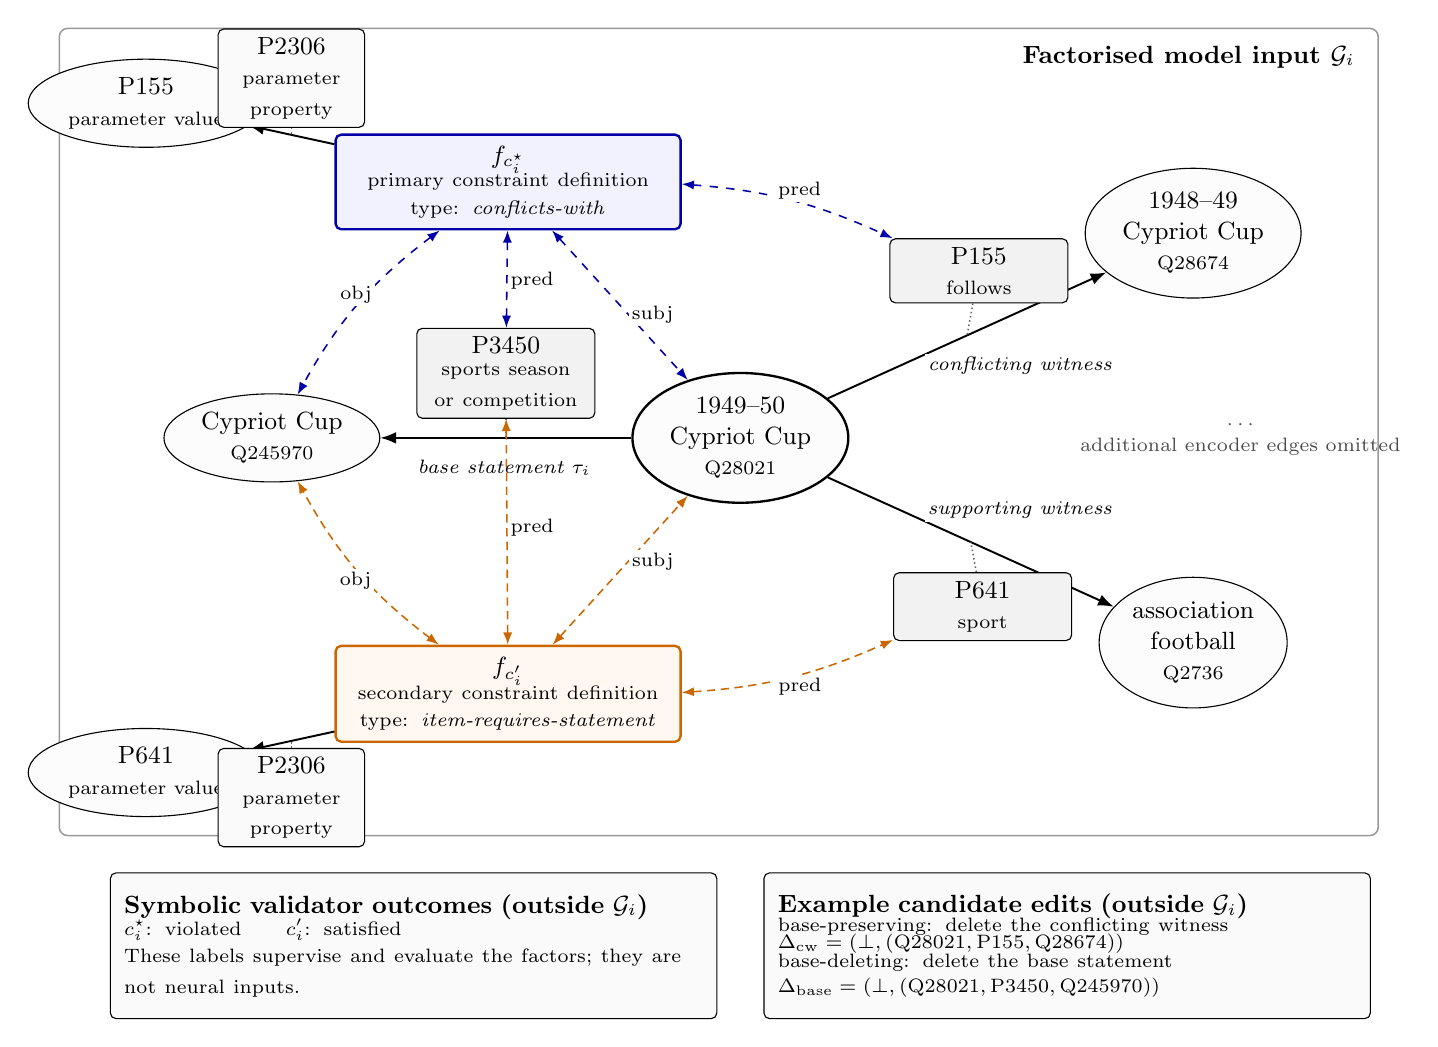
\begin{tikzpicture}[
  font=\small,
  term/.style={draw,ellipse,align=center,minimum width=2.15cm,minimum height=.95cm,inner sep=2pt,fill=black!1},
  focusitem/.style={term,line width=.85pt,minimum width=2.55cm,minimum height=1.15cm},
  pred/.style={draw,rounded corners=2pt,align=center,text width=2.05cm,minimum height=.70cm,inner sep=3pt,fill=black!5},
  parpred/.style={pred,text width=1.65cm,minimum height=.64cm,fill=black!2},
  factor/.style={draw,rounded corners=2pt,align=center,text width=4.10cm,minimum height=1.0cm,inner sep=4pt},
  primfactor/.style={factor,draw=blue!65!black,fill=blue!5,line width=.85pt},
  secfactor/.style={factor,draw=orange!80!black,fill=orange!6,line width=.85pt},
  outside/.style={draw,rounded corners=2pt,align=left,text width=7.35cm,minimum height=1.85cm,inner sep=5pt,fill=black!2},
  stredge/.style={-{Latex[length=2.0mm]},line width=.70pt},
  relattach/.style={densely dotted,draw=black!60,line width=.55pt},
  scopePrim/.style={{Latex[length=1.55mm]}-{Latex[length=1.55mm]},dashed,draw=blue!65!black,line width=.56pt},
  scopeSec/.style={{Latex[length=1.55mm]}-{Latex[length=1.55mm]},densely dashed,draw=orange!80!black,line width=.56pt},
  role/.style={font=\scriptsize,fill=white,inner sep=1.1pt,align=center},
  stmtrole/.style={font=\scriptsize\itshape,fill=white,inner sep=1.2pt},
  paneltitle/.style={font=\small\bfseries,fill=white,inner sep=1.5pt},
  note/.style={font=\scriptsize,align=center,text=black!70}
]
\draw[rounded corners=3pt,draw=black!40,line width=.55pt] (-8.65,-5.05) rectangle (8.10,5.20);
\node[paneltitle,anchor=north east] at (7.86,5.04) {Factorised model input $\mathcal{G}_i$};

\node[focusitem] (x) at (0,0) {1949--50\\Cypriot Cup\\\scriptsize Q28021};
\node[term] (cup) at (-5.95,0) {Cypriot Cup\\\scriptsize Q245970};
\path (x) -- coordinate[midway] (m3450) (cup);
\draw[stredge] (x) -- (cup);
\node[pred] (p3450) at ($(m3450)+(0,.82)$) {P3450\\\scriptsize sports season\\or competition};
\draw[relattach] (p3450) -- (m3450);
\node[stmtrole] at (-3.00,-.38) {base statement $\tau_i$};

\node[term] (prev) at (5.75,2.60) {1948--49\\Cypriot Cup\\\scriptsize Q28674};
\path (x) -- coordinate[midway] (m155) (prev);
\draw[stredge] (x) -- (prev);
\node[pred] (p155) at ($(m155)+(.15,.82)$) {P155\\\scriptsize follows};
\draw[relattach] (p155) -- (m155);
\node[stmtrole] at (3.55,.92) {conflicting witness};

\node[term] (football) at (5.75,-2.60) {association\\football\\\scriptsize Q2736};
\path (x) -- coordinate[midway] (m641) (football);
\draw[stredge] (x) -- (football);
\node[pred] (p641) at ($(m641)+(.15,-.82)$) {P641\\\scriptsize sport};
\draw[relattach] (p641) -- (m641);
\node[stmtrole] at (3.55,-.92) {supporting witness};
\node[note] at (6.35,0) {$\cdots$\\additional encoder edges omitted};

\node[primfactor] (fprim) at (-2.95,3.25) {\textbf{$f_{c_i^\star}$}\\[-1pt]\scriptsize primary constraint definition\\[-1pt]\scriptsize type: \emph{conflicts-with}};
\node[term,minimum width=1.75cm] (vprim) at (-7.55,4.25) {P155\\\scriptsize parameter value};
\path (fprim) -- coordinate[midway] (mqprim) (vprim);
\draw[stredge] (fprim) -- (vprim);
\node[parpred] (qprim) at ($(mqprim)+(0,.72)$) {P2306\\\scriptsize parameter property};
\draw[relattach] (qprim) -- (mqprim);
\draw[scopePrim] (fprim) -- node[role,right,pos=.56] {subj} (x);
\draw[scopePrim] (fprim) -- node[role,right,pos=.52] {pred} (p3450);
\draw[scopePrim] (fprim) to[bend right=12] node[role,above,pos=.52] {obj} (cup);
\draw[scopePrim] (fprim) to[bend left=10] node[role,above,pos=.55] {pred} (p155);

\node[secfactor] (fsec) at (-2.95,-3.25) {\textbf{$f_{c_i'}$}\\[-1pt]\scriptsize secondary constraint definition\\[-1pt]\scriptsize type: \emph{item-requires-statement}};
\node[term,minimum width=1.75cm] (vsec) at (-7.55,-4.25) {P641\\\scriptsize parameter value};
\path (fsec) -- coordinate[midway] (mqsec) (vsec);
\draw[stredge] (fsec) -- (vsec);
\node[parpred] (qsec) at ($(mqsec)+(0,-.72)$) {P2306\\\scriptsize parameter property};
\draw[relattach] (qsec) -- (mqsec);
\draw[scopeSec] (fsec) -- node[role,right,pos=.56] {subj} (x);
\draw[scopeSec] (fsec) -- node[role,right,pos=.52] {pred} (p3450);
\draw[scopeSec] (fsec) to[bend left=12] node[role,below,pos=.52] {obj} (cup);
\draw[scopeSec] (fsec) to[bend right=10] node[role,below,pos=.55] {pred} (p641);

\node[outside] (labels) at (-4.15,-6.45) {\textbf{Symbolic validator outcomes (outside $\mathcal{G}_i$)}\\[-1pt]\scriptsize $c_i^\star$: violated\qquad$c_i'$: satisfied\\[-1pt]\scriptsize These labels supervise and evaluate the factors; they are not neural inputs.};
\node[outside] (edits) at (4.15,-6.45) {\textbf{Example candidate edits (outside $\mathcal{G}_i$)}\\[-1pt]\scriptsize base-preserving: delete the conflicting witness\\[-2pt]\scriptsize $\Delta_{\mathrm{cw}}=(\bot,(\mathrm{Q28021},\mathrm{P155},\mathrm{Q28674}))$\\[-1pt]\scriptsize base-deleting: delete the base statement\\[-2pt]\scriptsize $\Delta_{\mathrm{base}}=(\bot,(\mathrm{Q28021},\mathrm{P3450},\mathrm{Q245970}))$};
\end{tikzpicture}%
}
\caption{A repair instance represented by the factorised model input \(\mathcal{G}_i\). Ellipses denote Wikidata term nodes, rounded grey boxes denote state-bearing predicate-occurrence nodes, and coloured boxes denote neural constraint factors. Solid arrows denote encoder edges, while the associated grey boxes denote their state-bearing predicate-occurrence nodes. %Dashed bidirectional links visualise membership in the role-specific factor scopes \(\mathcal{R}_{c,r}\), with \(r\in\{\mathrm{pred},\mathrm{subj},\mathrm{obj}\}\); they are used by the factor update rather than by the graph encoder.
}
\label{fig:subgraph-model}
\end{figure}

\subsection{Graph-encoder update}
\label{subsec:encoder-update}

Each node \(z\in\mathcal{Z}_i\) is associated with an entry in the model's global categorical vocabulary. For a Wikidata term node, this entry represents the corresponding item, property, or literal token. Predicate-occurrence nodes \(p_\tau\) and \(q_\theta\) use the entry of their underlying property \(p\) or \(q\), while a factor node \(f_c\) uses a synthetic entry associated with the concrete constraint definition \(c\). We denote the embedding retrieved from this vocabulary for node \(z\) by \(E_{\mathrm{cat}}(z)\).

Each node also receives a learned role embedding \(E_{\mathrm{role}}(z)\) indicating its role in the base statement \(\tau_i\). The role vocabulary distinguishes subject, predicate, and object nodes, includes a combined subject--object role when these coincide, and assigns a neutral role to all other nodes. The initial hidden state is
\[
h_z^{(0)}=\mathrm{MLP}_{\mathrm{init}}\left(E_{\mathrm{cat}}(z)\mathbin\Vert E_{\mathrm{role}}(z)\right).
\]
Distinct predicate-occurrence nodes representing the same underlying property therefore receive the same initial embedding, while remaining distinct nodes with separate hidden states.

The Direct--Factor GNN applies \(L\) encoder--factor blocks, indexed by \(k=0,\ldots,L-1\). At the beginning of block \(k\), \(h_z^{(k)}\) denotes the current state of node \(z\). Each block first applies a graph-encoder update, producing intermediate states \(\widetilde h_z^{(k+1)}\), and then a constraint-factor update, producing the states \(h_z^{(k+1)}\) passed to the next block.

For an encoder edge \(e=(u,\pi,v)\in\mathcal{E}_i^{\mathrm{enc}}\), an edge MLP transforms the hidden state of its predicate-occurrence node \(\pi\) into an edge feature:
\[
\epsilon_e^{(k)}=\mathrm{MLP}_{\mathrm{edge}}\left(h_\pi^{(k)}\right).
\]
The graph encoder then updates each node from its current state and its incoming encoder edges:
\[
\widetilde h_z^{(k+1)}=\mathrm{Enc}_k\left(h_z^{(k)},\left\{\left(h_u^{(k)},\epsilon_e^{(k)}\right):e=(u,\pi,z)\in\mathcal{E}_i^{\mathrm{enc}}\right\}\right).
\]

The intermediate states \(\widetilde h_z^{(k+1)}\) are then passed to the constraint-factor update described next. Nodes outside all factor scopes retain \(h_z^{(k+1)}=\widetilde h_z^{(k+1)}\), whereas nodes in factor scopes may receive a residual factor update.

\subsection{Constraint-factor read and write}
\label{subsec:factor-update}

This subsection describes the factor stage of each encoder--factor block. Each factor first aggregates the intermediate states in its role-specific scopes, computes a constraint-conditioned latent state, and then writes learned residual messages back to the nodes in those scopes. \Cref{fig:factor-architecture} summarises the resulting read--compute--write interface.

\begin{figure}[h]
\centering
\resizebox{0.97\textwidth}{!}{%
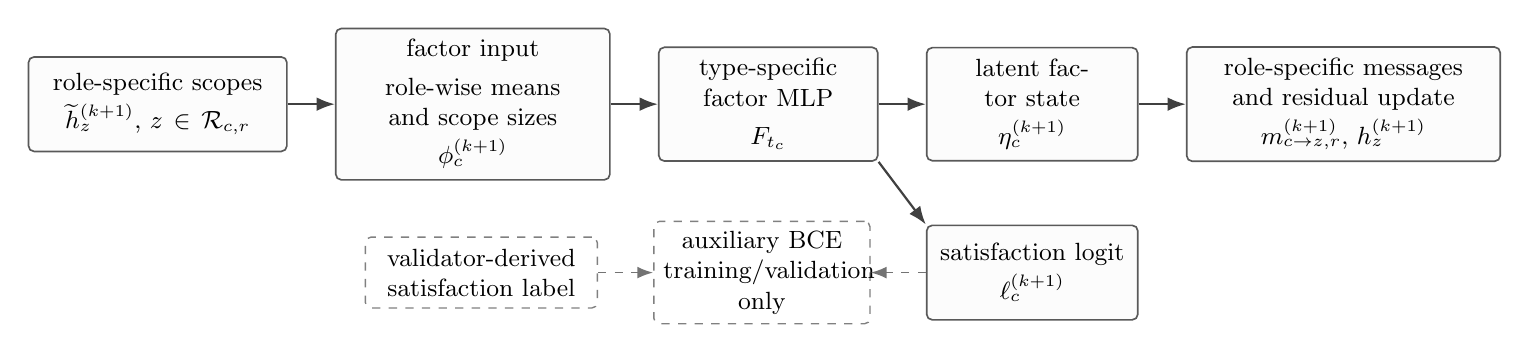
\begin{tikzpicture}[
  font=\small,
  >=Latex,
  main/.style={
    draw=black!65,
    rounded corners=2pt,
    line width=0.6pt,
    align=center,
    inner sep=4pt,
    minimum height=12mm,
    fill=black!1
  },
  aux/.style={
    draw=black!50,
    dashed,
    rounded corners=2pt,
    line width=0.5pt,
    align=center,
    inner sep=3.5pt,
    minimum height=9mm
  },
  flow/.style={
    ->,
    line width=0.8pt,
    draw=black!75
  },
  auxflow/.style={
    ->,
    dashed,
    line width=0.6pt,
    draw=black!55
  }
]

% Main factor-computation path
\node[main,text width=30mm] (scope) {
  role-specific scopes\\[1mm]
  $\widetilde h_z^{(k+1)}$,
  $z\in\mathcal R_{c,r}$
};

\node[main,text width=32mm,right=6mm of scope] (input) {
  factor input\\[1mm]
  role-wise means\\
  and scope sizes\\[1mm]
  $\phi_c^{(k+1)}$
};

\node[main,text width=25mm,right=6mm of input] (factor) {
  type-specific\\
  factor MLP\\[1mm]
  $F_{t_c}$
};

\node[main,text width=24mm,right=6mm of factor] (state) {
  latent factor state\\[1mm]
  $\eta_c^{(k+1)}$
};

\node[main,text width=37mm,right=6mm of state] (write) {
  role-specific messages\\
  and residual update\\[1mm]
  $m_{c\to z,r}^{(k+1)}$,
  $h_z^{(k+1)}$
};

\draw[flow] (scope) -- (input);
\draw[flow] (input) -- (factor);
\draw[flow] (factor) -- (state);
\draw[flow] (state) -- (write);

% Auxiliary supervision branch
\node[main,text width=24mm,below=8mm of state] (logit) {
  satisfaction logit\\[1mm]
  $\ell_c^{(k+1)}$
};

\node[aux,text width=25mm,left=7mm of logit] (loss) {
  auxiliary BCE\\
  training/validation only
};

\node[aux,text width=27mm,left=7mm of loss] (label) {
  validator-derived\\
  satisfaction label
};

\draw[flow] (factor.south east) -- (logit.north west);
\draw[auxflow] (label) -- (loss);
\draw[auxflow] (logit) -- (loss);

\end{tikzpicture}%
}
\caption{Read--compute--write interface of a neural constraint factor. Solid arrows show the factor computation and residual message pathway; dashed arrows show the auxiliary validator supervision used during training and validation.}
\label{fig:factor-architecture}
\end{figure}

For each factor \(f_c\) and role \(r\in\mathsf{Role}\), the scope \(\mathcal{R}_{c,r}\) of the factor may contain zero, one, or several nodes. After the graph-encoder update, the factor computes a separate mean representation for each role:
\[
\bar h_{c,r}^{(k+1)}=\frac{1}{\max(1,|\mathcal{R}_{c,r}|)}\sum_{z\in\mathcal{R}_{c,r}}\widetilde h_z^{(k+1)}.
\]
The summary is the zero vector when the scope is empty. The factor input concatenates the intermediate factor-node state, the three role summaries, and the logarithm of each scope size:
\[
\phi_c^{(k+1)}=\left[\widetilde h_{f_c}^{(k+1)}\mathbin\Vert\bar h_{c,\mathrm{pred}}^{(k+1)}\mathbin\Vert\bar h_{c,\mathrm{subj}}^{(k+1)}\mathbin\Vert\bar h_{c,\mathrm{obj}}^{(k+1)}\mathbin\Vert\log(1+|\mathcal{R}_{c,\mathrm{pred}}|)\mathbin\Vert\log(1+|\mathcal{R}_{c,\mathrm{subj}}|)\mathbin\Vert\log(1+|\mathcal{R}_{c,\mathrm{obj}}|)\right].
\]
The scope-size features distinguish an empty role from one containing one or several local nodes.

Factors representing definitions of the same constraint type share a type-specific two-layer MLP \(F_{t_c}\), allowing the computation to specialise by constraint type while sharing parameters across factors of that type. It maps the factor input to a latent factor state \(\eta_c^{(k+1)}\) and a constraint-satisfaction logit \(\ell_c^{(k+1)}\):
\[
\bigl(\eta_c^{(k+1)},\ell_c^{(k+1)}\bigr)=F_{t_c}\left(\phi_c^{(k+1)}\right).
\]

During training, each satisfaction logit is supervised by the symbolic validator label when the factor's local evaluation is checkable. The factor MLP is thereby trained to approximate the validator's satisfaction judgement from the representations available in its scope. The satisfaction logit serves only as this auxiliary prediction; the latent state \(\eta_c^{(k+1)}\) drives factor communication.

After the final encoder--factor block, the same factor MLP is applied once more to the completed node states to obtain the final factor readout \(\eta_c^{\mathrm{out}}\) and the final satisfaction logit \(\ell_c\) used by the auxiliary loss below.

For each node \(z\in\mathcal{R}_{c,r}\), a type- and role-specific MLP \(M_{t_c,r}\) creates a message from the factor state and the recipient's intermediate state:
\[
m_{c\to z,r}^{(k+1)}=M_{t_c,r}\left(\eta_c^{(k+1)}\mathbin\Vert\widetilde h_z^{(k+1)}\right).
\]
Messages arriving at the same node are averaged and added as a residual:
\[
h_z^{(k+1)}=\widetilde h_z^{(k+1)}+\lambda\frac{\displaystyle\sum_{(c,r):z\in\mathcal{R}_{c,r}}m_{c\to z,r}^{(k+1)}}{\max(1,d_z)},
\qquad
d_z=\bigl|\{(c,r):z\in\mathcal{R}_{c,r}\}\bigr|.
\]

Nodes outside all factor scopes retain \(h_z^{(k+1)}=\widetilde h_z^{(k+1)}\). Together with the preceding graph-encoder update, the residual write-back completes encoder--factor block \(k\), and the resulting states become the inputs to the next block.

\subsection{Edit prediction and training signals}
\label{subsec:edit-decoding}

This subsection describes how the final node states are decoded into the predicted edit \(\prededit_i\) and how the historical edit \(\histedit_i\) and symbolic validator outcomes provide the training signals for the Direct--Factor GNN.

\paragraph*{Six-slot decoding.} After the final encoder--factor block, the model mean-pools the node states \(h_z^{(L)}\) to obtain a graph-level representation of repair instance \(i\). The pooled graph representation is first transformed by a shared linear projection and then by three separate subject, predicate, and object branches, each implemented as a linear layer with LeakyReLU activation. Each branch feeds separate addition and deletion heads, yielding six output logits \(\mathbf{s}_{i,j}, \: j\in\{1,\dots, 6\}.\) At inference, the highest-scoring value is selected independently in every slot producing the model's prediction \(\prededit_i.\)

\paragraph*{Training signals.} The primary objective is to reproduce the historical edit \(\histedit_i\). Its six-slot encoding \(y(\histedit_i)\) provides one categorical target for each decoder head, giving the edit-prediction loss
\[
\mathcal{L}_{\mathrm{edit}}^{(i)}
=
\frac{1}{6}
\sum_{j=1}^{6}
\mathrm{CE}\!\left(
\mathbf{s}_{i,j},
y_j(\histedit_i)
\right).
\]

The Direct--Factor GNN additionally receives two auxiliary satisfaction signals derived from the symbolic validators. The final factor readout predicts whether each checkable constraint definition is satisfied on the pre-edit state \(G_i^{\mathrm{pre}}\). A second, training-only head predicts satisfaction after the historical edit: it receives the final factor representation together with the mean learned embedding of the six slots of \(y(\histedit_i)\) and is supervised against the validator outcome on \(G_i^{\mathrm{hist}}\). We denote the corresponding binary-cross-entropy losses, averaged only over constraint definitions that are checkable in the relevant state, by \(\overline{\mathrm{BCE}}_{\mathrm{pre}}^{(i)}\) and \(\overline{\mathrm{BCE}}_{\mathrm{hist}}^{(i)}\), respectively.

For the reported Direct--Factor configuration, the complete per-instance training loss is
\[
\mathcal{L}_{\mathrm{DF}}^{(i)}
=
\mathcal{L}_{\mathrm{edit}}^{(i)}
+
0.1\,\overline{\mathrm{BCE}}_{\mathrm{pre}}^{(i)}
+
0.1\,\overline{\mathrm{BCE}}_{\mathrm{hist}}^{(i)}.
\]
An auxiliary term is zero when no constraint definition is checkable for its corresponding state. The historical edit is used by the post-historical-edit head only during training and validation and is never supplied to the model at inference. The auxiliary satisfaction predictions shape the factor pathway but are not inputs to the edit decoder. Constraint-satisfaction metrics are instead computed by applying \(\prededit_i\) to \(G_i^{\mathrm{pre}}\) and independently running the symbolic validators on the resulting state, as described in \cref{sec:evaluation}.

\subsection{Why neural constraint factors?}
\label{subsec:what-factors-measure}

Representing a constraint definition only through encoder edges leaves a generic graph encoder to discover which local nodes fill different semantic roles and how their evidence should be combined for each constraint type. Neural constraint factors encode this inductive bias directly: each factor reads role-specific scopes and returns constraint-conditioned residuals to the nodes in those scopes, using modules shared by factors of the same constraint type. This gives constraint information a direct pathway into the edit representation without prescribing a symbolic edit or invoking a validator during neural inference.

The explicit interface also makes the constraint pathway easier to interrogate. Satisfaction probes test whether factor states encode their symbolic satisfaction labels, while factor-message-masking interventions test whether messages from primary and secondary factors affect the predicted edit. These diagnostics distinguish label alignment from pathway use; neither establishes validator-equivalent reasoning or repair safety. Those outcomes require the post-edit symbolic evaluation defined in \cref{sec:evaluation}.

\section{Evaluation Framework}
\label{sec:evaluation}

Historical fidelity compares the predicted edit\(\prededit_i\) with the historical recorded edit \(\histedit_i\): \textbf{precision, recall, and Micro-F1} pool are computed on their additions and deletions. Constraint-satisfaction metrics instead compare the symbolic states resulting to applying the edits \(G_i^{\mathrm{pre}}\) and \(G_i^{\mathrm{pred}}\).

\paragraph*{Constraint support.} The type-specific validators in \cref{tab:validator-semantics} produce the outcomes used here. For each instance \(i\) and factor-supported definition \(c\in\mathcal{C}_i^{\mathrm{fac}}\), let \(\chi_c(G)\in\{0,1\}\) indicate whether its local evaluation is checkable on \(G\). When it is checkable, let \(\sigma_c(G)\in\{0,1\}\) indicate whether the definition is satisfied. The same Wikidata constraint definition may be selected in multiple repair instances, so each pair \((i,c)\) constitutes a distinct local constraint evaluation; the instance index is omitted from \(\chi_c\) and \(\sigma_c\) for readability. Define the post-edit and common supports as
\[
\mathcal{C}_i^{\mathrm{pred}}
=\{c\in\mathcal{C}_i^{\mathrm{fac}}:\chi_c(\Gpred)=1\},\quad
\mathcal{C}_i^{\leftrightarrow}
=\{c\in\mathcal{C}_i^{\mathrm{fac}}:\chi_c(\Gpre)=1\land\chi_c(\Gpred)=1\}.
\]
We call \(\mathcal{C}_i^{\leftrightarrow}\) the \emph{common support}: it contains exactly those constraint definitions whose local evaluations are checkable both before and after the predicted edit, so their satisfaction values can be compared.
Every constraint-satisfaction metric reports its eligible denominator; an uncheckable local evaluation contributes neither a positive result nor an artificial zero.

\paragraph*{Primary and local satisfaction.}
Let the Primary-Fix eligibility set be the set of instances whose primary constraint definition is checkable and violated before the edit.
\[
\mathcal{I}_{\mathrm{PF}}
=
\left\{
i:
\chi_{c_i^\star}(\Gpre)=1
\land
\sigma_{c_i^\star}(\Gpre)=0
\right\}.
\]
The \textbf{Primary Fix Rate (PFR)} measures the proportion of eligible instances whose primary constraint definition is fixed by the system's predicted edit.
\[
\mathrm{PFR}=
\frac{\sum_{i\in\mathcal{I}_{\mathrm{PF}}}
\mathbf{1}[\chi_{c_i^\star}(\Gpred)=1\land \sigma_{c_i^\star}(\Gpred)=1]}
{|\mathcal{I}_{\mathrm{PF}}|}.
\]
\textbf{Post-edit Local Satisfaction} \(\locsat^{\mathrm{pred}}\) is the proportion of checkable post-edit local constraint evaluations that are satisfied, while the \textbf{Change in Local Satisfaction} \(\Delta\locsat\) uses common support so altered coverage is not mistaken for improvement:
\[
\locsat^{\mathrm{pred}}=
\frac{\sum_i\sum_{c\in\mathcal{C}_i^{\mathrm{pred}}}\sigma_c(\Gpred)}
{\sum_i|\mathcal{C}_i^{\mathrm{pred}}|},
\qquad
\Delta\locsat=
\frac{\sum_i\sum_{c\in\mathcal{C}_i^{\leftrightarrow}}
[\sigma_c(\Gpred)-\sigma_c(\Gpre)]}
{\sum_i|\mathcal{C}_i^{\leftrightarrow}|}.
\]

\paragraph*{Secondary satisfaction.}
For secondary satisfaction, exclude the primary constraint definition from the common support \(\mathcal{C}_i^{\mathrm{sec}} =\mathcal{C}_i^{\leftrightarrow}\setminus\{c_i^\star\}.\)
The \textbf{Secondary Improvement Rate (SIR)} and \textbf{Secondary Regression Rate (SRR)} are computed over eligible definition--instance pairs. SIR measures how often a secondary constraint definition that is violated before the edit becomes satisfied, while SRR measures the converse transition from satisfied to violated:
\[
\begin{aligned}
\sir
&=\frac{\sum_i\sum_{c\in\mathcal{C}_i^{\mathrm{sec}}}
\mathbf{1}[\sigma_c(\Gpre)=0\land \sigma_c(\Gpred)=1]}
{\sum_i\sum_{c\in\mathcal{C}_i^{\mathrm{sec}}}\mathbf{1}[\sigma_c(\Gpre)=0]},\\
\srr
&=\frac{\sum_i\sum_{c\in\mathcal{C}_i^{\mathrm{sec}}}
\mathbf{1}[\sigma_c(\Gpre)=1\land \sigma_c(\Gpred)=0]}
{\sum_i\sum_{c\in\mathcal{C}_i^{\mathrm{sec}}}\mathbf{1}[\sigma_c(\Gpre)=1]}.
\end{aligned}
\]
An instance with no secondary constraint definition eligible for SIR or SRR is excluded from the corresponding computations rather than being assigned a value of zero.

\paragraph*{Edit size and base-statement preservation.}
Constraint satisfaction alone does not reveal how an edit achieved its score: a targeted correction, a multi-operation rewrite, and removal of the statement witnessing the violation may all improve local validation outcomes. We therefore complement the satisfaction metrics with diagnostics of operation count and base-statement preservation.

\textbf{Edit size} is the number of operations in the predicted edit \(\prededit_i\). Because an edit contains at most one addition and one deletion, its size lies in \(\{0,1,2\}\). We report the mean edit size together with the separate \textbf{mean addition and deletion counts}.

Because the base statement \(\tau_i\) is present in \(\Gpre\), its absence from \(\Gpred\) indicates that it was removed by the predicted edit. The \textbf{Base-removal Rate} is the fraction of instances for which \(\tau_i\notin\Gpred\).

The \textbf{Base-Preserving Primary Fix rate (BPPF)} measures how often an eligible primary violation is fixed while retaining the base statement:
\[
\bppf
=\frac{\sum_{i\in\mathcal{I}_{\mathrm{PF}}}
\mathbf{1}[\chi_{c_i^\star}(\Gpred)=1
\land \sigma_{c_i^\star}(\Gpred)=1
\land \tau_i\in\Gpred]}
{|\mathcal{I}_{\mathrm{PF}}|}.
\]

The \textbf{Base-removal-and-improvement Rate} measures the fraction of all test instances in which the predicted edit both removes the base statement and produces a positive net change in satisfaction over the common support, that is, \(\tau_i\notin\Gpred\) and \(\sum_{c\in\mathcal{C}_i^{\leftrightarrow}}[\sigma_c(\Gpred)-\sigma_c(\Gpre)]>0\). An empty common support has net change zero and therefore does not count as an improvement.

Together, these diagnostics distinguish frequent base removal, primary fixes that preserve the base statement, and satisfaction improvements that coincide with base removal.

\section{Experimental Setup}
\label{sec:experiments}

\subsection{Benchmark and constraint coverage}
\label{sec:benchmark}

We construct the benchmark from 1,910,794 correction records in the corpus of Pellissier Tanon dt al. \cite{pellissier2019learning,pellissier2021neural}, extracted from the 1 July 2018 Wikidata full-history dump. Each retained record is converted into the repair-instance representation of \cref{sec:task:instance}: the recorded violation supplies the primary constraint definition and the recorded historical edit, while the supplied local entity descriptions form the bounded A-box neighbourhood. We additionally select constraint definitions for locally represented properties, yielding secondary definitions alongside the primary one. All retained historical edits fit the six-slot encoding of \cref{sec:task:action} without truncation.

We partition correction rows 70/15/15 by primary constraint type and then retain a 50\% stratified subsample preserving the distributions of split, primary constraint type, and local constraint-definition count. The resulting benchmark contains 955,405 instances: 668,779 for training, 143,310 for validation, and 143,316 for testing. %The split unit is a correction row rather than an entity or concrete constraint definition, so both may recur across partitions; the resulting in-distribution evaluation scope is discussed in \cref{sec:discussion}.

\begin{table}[h]
\caption{Per-instance descriptive statistics for the 143,316 held-out test cases. A-box counts use distinct statements in the pre-edit state.}
\label{tab:benchmark-statistics}
\centering
\small
\begin{tabularx}{\textwidth}{@{}Xrrrr@{}}
\toprule
\textbf{Quantity} & \textbf{Mean} & \textbf{Median} & \textbf{95th pct.} & \textbf{Max.} \\
\midrule
Local A-box statements & 26.55 & 17 & 74 & 558 \\
Local constraint definitions & 101.05 & 83 & 266 & 1,092 \\
Neural constraint factors & 60.60 & 51 & 168 & 662 \\
\bottomrule
\end{tabularx}
\end{table}

\label{sec:constraint-types}
The primary constraint definitions represented by neural factors span the following types: conflicts-with, distinct-values, inverse, item-requires-statement, one-of, single-value, subject type, value-requires-statement, and value-type. Symmetric appears only among secondary factors. A constraint definition is represented as a neural constraint factor when its local validator
(\cref{tab:validator-semantics}) is supported. Other local constraint definitions
remain descriptive metadata and do not contribute Boolean satisfaction outcomes.

Among factor-supported definition--instance pairs, 64.9\% are checkable in the pre-edit state and 67.9\%
after applying the historical edit. Checkable local evaluations provide the symbolic targets used to
supervise the auxiliary satisfaction heads.

\subsection{Proposal architectures and baselines}
\label{subsec:models-baselines}
The Direct group contains two neural systems whose six output slots are decoded independently. The Direct--Factor GNN is the neural-constraint-factor architecture described in \cref{sec:neural-constraint-factors}; it uses type-specific factor MLPs, factor messages, and auxiliary satisfaction heads. The Direct--Passive GNN is the neural baseline and uses a passive GINE encoder. Its graph retains the primary constraint-definition branch but has no neural constraint-factor scopes, auxiliary satisfaction heads, or factor messages.

The Baseline group contains four non-neural comparators. Baseline--DB (Delete Base) and Baseline--AM (Add Mirror) are deterministic symbolic heuristics. Baseline--DB always deletes \(\tau_i\). For inverse and symmetric constraint types, Baseline--AM reverses the base statement, using a known inverse property when available and otherwise retaining the original property; it predicts no edit for other constraint types. Baseline--CTM (Constraint-Type Majority) and Baseline--DM (Definition Majority) are statistical: each predicts the most frequent training target independently for every action slot, conditioned on the constraint type or concrete constraint definition, respectively.

\subsection{Decision-level candidate systems}
\label{subsec:decision-variants}

The Direct--Factor GNN gives constraint information a pathway into the edit representation, but its six heads choose slot values independently and do not compare complete edits by their constraint consequences. Candidate-level decision mechanisms let us probe the fidelity--safety gap more directly by selecting among complete candidate edits under objectives that place different weight on historical agreement and post-edit constraint behaviour. Comparing these systems reveals whether improvements in validator-based outcomes come at the expense of historical fidelity or evidence preservation, and whether satisfaction-oriented selection admits degenerate repair strategies.

The two Direct systems each decode one edit from six independently predicted slots. Candidate--C (Chooser), Candidate--DP (Direct Penalty), and Candidate--SR (Satisfaction Reranker) instead choose from a candidate set \(\Gamma_i=\{\Delta_{ij}\}_{j=1}^{|\Gamma_i|}\) derived from proposal logits and constraint heuristics, where \(\Delta_{ij}\) denotes candidate edit \(j\) for instance \(i\). Applying a candidate to the pre-edit state yields \(G_{ij}=\operatorname{apply}(\Gpre,\Delta_{ij})\). Let \(\alpha_{ij}\) be the raw selection score of \(\Delta_{ij}\). All three systems normalise over the candidates of an instance as \(\pi_{ij}=\exp(\alpha_{ij})/\sum_{k=1}^{|\Gamma_i|}\exp(\alpha_{ik})\). Candidate--C and Candidate--SR learn \(\alpha_{ij}\); for Candidate--DP it is the sum of the six proposal logits selected by \(\Delta_{ij}\). During training and validation, the recorded historical edit is additionally inserted into the candidate set. When present, let \(j_i^{\mathrm{hist}}\) denote its index, so that \(\Delta_{i j_i^{\mathrm{hist}}}=\histedit_i\).

For candidate edit \(\Delta_{ij}\), the primary-fix indicator is \(\sigma_{ij}^{\mathrm{prim}}=\mathbf{1}[\chi_{c_i^\star}(G_{ij})=1\land \sigma_{c_i^\star}(G_{ij})=1]\), so making the primary constraint definition uncheckable counts as a failure. Secondary regression is likewise evaluated for the state induced by \(\Delta_{ij}\), relative to the pre-edit state rather than the historical post-edit state. Specifically, let
\[
\mathcal{C}_{ij}^{\mathrm{sec}}=
\{c\in\mathcal{C}_i\setminus\{c_i^\star\}:
\chi_c(\Gpre)=\chi_c(G_{ij})=1\}.
\]
Then
\[
\mathrm{SRR}_{ij}^{\mathrm{cand}}=
\frac{
\sum_{c\in\mathcal{C}_{ij}^{\mathrm{sec}}}
\mathbf{1}[\sigma_c(\Gpre)=1\land \sigma_c(G_{ij})=0]
}{
\sum_{c\in\mathcal{C}_{ij}^{\mathrm{sec}}}
\mathbf{1}[\sigma_c(\Gpre)=1]
},
\]
with value zero when the denominator is empty. Each candidate edit therefore has its own common support. For the historical candidate, these quantities are obtained by setting \(j=j_i^{\mathrm{hist}}\).

Candidate--C adds a learned chooser whose goal is to select the recorded historical edit while favouring primary fixes and discouraging secondary regressions beyond those caused by that edit. It scores each candidate \(\Delta_{ij}\) from the Direct--Factor GNN graph embedding and the mean learned embedding of its six slot IDs. In addition to \(\mathcal{L}_{\mathrm{factor}}^{(i)}\), it uses
\[
0.25\!\left[
-\log \pi_{i,j_i^{\mathrm{hist}}}
+0.25\sum_j \pi_{ij}\max\!\left(
0,
\mathrm{SRR}_{ij}^{\mathrm{cand}}-
\mathrm{SRR}_{i,j_i^{\mathrm{hist}}}^{\mathrm{cand}}
\right)
+0.2\sum_j \pi_{ij}(1-\sigma_{ij}^{\mathrm{prim}})
\right].
\]

Candidate--DP has no separate chooser: it derives candidate probabilities directly from the proposal slot logits and trains the proposal model itself to favour primary fixes with fewer secondary regressions. It adds the expected penalty
\[
\sum_j\pi_{ij}(1-\sigma_{ij}^{\mathrm{prim}})
+0.5\sum_j\pi_{ij}\mathrm{SRR}_{ij}^{\mathrm{cand}}.
\]
Candidate--SR is deliberately satisfaction-only: it keeps the Direct--Factor GNN frozen for candidate generation and trains a separate graph encoder and candidate reranker to prefer candidates with the highest satisfaction rate over checkable local constraint evaluations. It minimises
\[
\mathcal{L}_{\mathrm{SR}}^{(i)}=-\sum_j\pi_{ij}\bar\sigma_{ij},
\]
where \(\bar\sigma_{ij}=|\{c\in\mathcal{C}_i:\chi_c(G_{ij})=1\land \sigma_c(G_{ij})=1\}|/|\{c\in\mathcal{C}_i:\chi_c(G_{ij})=1\}|\), defined as zero when no local constraint is checkable. Because the denominator and candidate SRR support depend on \(G_{ij}\), making a constraint uncheckable can remove it from either quantity; in particular, removing violated constraints can raise \(\bar\sigma_{ij}\). This vulnerability is the purpose of the Candidate--SR diagnostic. At inference, Candidate--C and Candidate--SR use learned-score argmax, while Candidate--DP uses proposal-logit argmax. These candidate-level terms are instance-normalised training quantities, not the evaluation-pooled metrics in \cref{sec:evaluation}.

\subsection{Optimisation and candidate construction}
\label{subsec:training-protocol}

The Direct--Factor GNN, Candidate--C, and Candidate--DP use 400-dimensional hidden states and three GINE--factor blocks%, whereas the Direct--Passive GNN uses 128-dimensional states and one GINE block
. All learned systems are trained with Adam and selected by validation loss. Candidate--C and Candidate--DP are trained jointly with the Direct--Factor proposal model; Candidate--SR instead freezes that proposal model and trains a separate candidate reranker. Full optimisation and architecture hyperparameters are reported in the supplementary reproducibility appendix.

Candidate sets combine high-scoring single-add and single-delete actions from the proposal model with instantiated constraint heuristics. After deduplication, each inference set is capped at 80 candidates. The recorded historical edit is inserted only into candidate sets used to compute training and validation losses. At inference, including for candidate-oracle analysis, candidate sets are constructed without access to \(\histedit\).

\subsection{Evaluation protocol}
\label{subsec:evaluation-protocol}

All reported test metrics use a common symbolic reconstruction procedure. For each instance, we reconstruct the pre-edit state by merging graph roles that denote the same entity and ensuring that the base statement \(\tau_i\) is present; predicted edits are then applied with deletion preceding addition. Checkability and satisfaction are recomputed on the resulting post-edit state. Candidate-level symbolic objectives used during training follow the model-specific reconstruction procedures documented in the supplementary reproducibility appendix, but these differences do not affect the common evaluation used for the reported results. Each aggregate metric is accompanied by its numerator and denominator, and no test metric is used for model selection.

\begin{table}[H]
\caption{Pre-edit state of the primary constraint definition on the full test split. PFR and BPPF use the checkable-and-violated row as a fixed eligibility set; all 143,316 predictions remain in the evaluation.}
\label{tab:primary-eligibility}
\centering
\small
\begin{tabular}{lrr}
\toprule
\textbf{Pre-edit primary state} & \textbf{Instances} & \textbf{Share} \\
\midrule
Checkable and violated (eligible) & 54,234 & 37.84\% \\
Uncheckable from local evidence & 39,781 & 27.76\% \\
Checkable but already satisfied & 49,301 & 34.40\% \\
\midrule
Total & 143,316 & 100.00\% \\
\bottomrule
\end{tabular}
\end{table}

PFR and BPPF are therefore evaluated on the 54,234 instances whose primary constraint definition is checkable and violated before the edit. Instances with insufficient local evidence or an already satisfied primary definition do not represent a locally reproduced primary violation that the predicted edit can meaningfully fix and are excluded from these denominators. If an eligible primary becomes uncheckable after the predicted edit, it counts as a failure rather than leaving the fixed eligibility set.


\section{Results}
\label{sec:results}

\subsection{Historical fidelity and symbolic behaviour diverge}
\label{subsec:aggregate-results}

The aggregate results do not induce a single model ranking. The system that best reproduces historical edits is not the one that most often satisfies the primary validator, and improvements in local satisfaction can coincide with more aggressive evidence removal. We therefore interpret \cref{tab:main-results,tab:symbolic-results,tab:transition-results} as complementary views of predicted-edit behaviour rather than interchangeable measures of quality. Arrows in table headers indicate the preferred direction; unmarked columns are descriptive. Bold and underlined values mark the best and second-best results, respectively.

\begin{table}[h]
\caption{Historical fidelity and predicted edit size. Add and Del are the mean numbers of complete addition and deletion operations predicted per instance.}
\label{tab:main-results}
\centering
\small
\begin{tabular}{lrrrrrr}
\toprule
\textbf{Model} & \textbf{Precision \(\uparrow\)} & \textbf{Recall \(\uparrow\)} & \textbf{Micro-F1 \(\uparrow\)} & \textbf{Add} & \textbf{Del} & \textbf{Edit size \(\downarrow\)} \\
\midrule
Direct--Passive GNN & 0.5659 & 0.5296 & 0.5471 & 0.5159 & 0.4821 & 0.9979 \\
Direct--Factor GNN  & \textbf{0.6890} & \textbf{0.6689} & \textbf{0.6788} & 0.5747 & 0.4604 & 1.0352 \\
\midrule
Candidate--C  & 0.5318 & 0.4988 & 0.5148 & 0.5676 & 0.4324 & 1.0000 \\
Candidate--DP & 0.4528 & 0.4222 & 0.4370 & 0.5326 & 0.4617 & \underline{0.9943} \\
Candidate--SR & 0.2726 & 0.2557 & 0.2639 & 0.0000 & 1.0000 & 1.0000 \\
\midrule
Baseline--DB & 0.2897 & 0.2717 & 0.2804 & 0.0000 & 1.0000 & 1.0000 \\
Baseline--AM & 0.2814 & 0.0276 & 0.0503 & 0.1047 & 0.0000 & \textbf{0.1047} \\
Baseline--CTM & 0.2732 & 0.2580 & 0.2654 & 0.5305 & 0.4766 & 1.0072 \\
Baseline--DM & \underline{0.6563} & \underline{0.6404} & \underline{0.6482} & 0.5603 & 0.4801 & 1.0404 \\
\bottomrule
\end{tabular}
\end{table}

At the system level, the Direct--Factor GNN exceeds the Direct--Passive GNN by 0.1317 Micro-F1 while predicting only 0.0373 more operations per instance, so the fidelity difference is not explained by indiscriminately producing more edits. Baseline--DM is nevertheless only 0.0306 behind the factor model. Because concrete constraint definitions may recur across the random split, this result shows that definition identity is a strong predictor of historical curator actions in this in-distribution setting; it should not be interpreted as evidence of generalisation to unseen definitions. 

\begin{table}[h]
\caption{Primary, local, and base-statement-preservation metrics. \(n_{\locsat}\) and \(n_{\delta}\) count eligible local constraint evaluations. BaseRem denotes base-removal rate, BaseDelAct base-deletion-action rate, and BaseRemImp base-removal-associated-improvement rate.}
\label{tab:symbolic-results}
\centering
\scriptsize
\resizebox{\textwidth}{!}{%
\begin{tabular}{lrrrrrrrrr}
\toprule
\textbf{Model} & \textbf{PFR \(\uparrow\)} & \textbf{LocalSat \(\uparrow\)} & \(n_{\locsat}\) & \(\Delta\locsat\,\uparrow\) & \(n_{\delta}\) & \textbf{BaseRem \(\downarrow\)} & \textbf{BaseDelAct \(\downarrow\)} & \textbf{BPPF \(\uparrow\)} & \textbf{BaseRemImp \(\downarrow\)} \\
\midrule
Direct--Passive GNN & 0.8109 & 0.7622 & 5,322,054 & 0.0201 & 4,691,844 & 0.4342 & 0.4345 & \underline{0.1201} & 0.3419 \\
Direct--Factor GNN  & 0.6278 & 0.7518 & 5,189,194 & 0.0154 & 4,691,910 & 0.3517 & 0.3622 & 0.1053 & 0.2702 \\
\midrule
Candidate--C  & 0.5950 & 0.7490 & 5,127,377 & 0.0156 & 4,691,615 & \underline{0.3121} & \underline{0.3121} & 0.1026 & \underline{0.2364} \\
Candidate--DP & 0.7707 & 0.7628 & 5,331,576 & 0.0202 & 4,692,049 & 0.4442 & 0.4442 & 0.0350 & 0.3576 \\
Candidate--SR & \underline{0.9200} & \textbf{0.8021} & 5,931,955 & \textbf{0.0394} & 4,689,235 & 0.9741 & 0.9741 & 0.0604 & 0.5659 \\
\midrule
Baseline--DB & \textbf{0.9218} & \underline{0.7995} & 5,962,474 & \underline{0.0349} & 4,690,179 & 1.0000 & 1.0000 & 0.0000 & 0.5782 \\
Baseline--AM & 0.0148 & 0.7105 & 4,692,077 & 0.0002 & 4,692,077 & \textbf{0.0000} & \textbf{0.0000} & 0.0148 & \textbf{0.0000} \\
Baseline--CTM & 0.6719 & 0.7530 & 5,217,600 & 0.0152 & 4,691,561 & 0.3713 & 0.3714 & 0.1192 & 0.2891 \\
Baseline--DM & 0.8037 & 0.7589 & 5,280,993 & 0.0185 & 4,691,750 & 0.4078 & 0.4166 & \textbf{0.1462} & 0.3229 \\
\bottomrule
\end{tabular}%
}
\end{table}

The fidelity advantage does not transfer to bounded symbolic outcomes. The Direct--Passive GNN fixes substantially more eligible primaries than the Direct--Factor GNN, but also removes the base statement 8.25 percentage points more often and produces 7.17 points more base-removal-associated improvements. The Direct--Factor GNN therefore preserves the base statement more often, yet leaves more primary violations unresolved. Neither system dominates: the passive system obtains stronger validator outcomes partly through more deletion, whereas the factor system achieves higher curator agreement with less evidence removal.

Candidate--DP demonstrates that decision-level penalties can move the targeted rule metrics. Relative to the Direct--Factor GNN, it raises PFR by 14.29 points, raises SIR by 0.93 points, and lowers SRR by 0.09 points. These changes cost 24.18 points of Micro-F1, increase base removal by 9.25 points, and reduce BPPF by 7.03 points. The extra primary fixes therefore do not constitute a general safety improvement: most of the gain disappears once retention of the base statement is required. Candidate--C occupies a more conservative point, with the lowest base-removal and base-removal-associated-improvement rates among learned systems, but it improves neither fidelity nor primary fixing over the Direct--Factor GNN.

\begin{table}[h]
\caption{Evaluation-pooled secondary satisfaction transitions. The \(n\) columns count eligible definition--instance pairs.}
\label{tab:transition-results}
\centering
\small
\begin{tabular}{lrrrr}
\toprule
\textbf{Model} & \textbf{SIR \(\uparrow\)} & \(n_{\mathrm{SIR}}\) & \textbf{SRR \(\downarrow\)} & \(n_{\mathrm{SRR}}\) \\
\midrule
Direct--Passive GNN & 0.0521 & 1,305,030 & 0.0053 & 3,283,279 \\
Direct--Factor GNN  & 0.0413 & 1,305,024 & 0.0048 & 3,283,351 \\
\midrule
Candidate--C  & 0.0417 & 1,304,991 & 0.0041 & 3,283,089 \\
Candidate--DP & 0.0506 & 1,305,021 & \underline{0.0039} & 3,283,493 \\
Candidate--SR & \textbf{0.1221} & 1,304,470 & 0.0074 & 3,281,230 \\
\midrule
Baseline--DB & \underline{0.1113} & 1,304,929 & 0.0095 & 3,281,715 \\
Baseline--AM & 0.0000 & 1,305,033 & \textbf{0.0000} & 3,283,509 \\
Baseline--CTM & 0.0392 & 1,305,031 & 0.0049 & 3,282,995 \\
Baseline--DM & 0.0483 & 1,304,998 & 0.0060 & 3,283,217 \\
\bottomrule
\end{tabular}
\end{table}


The secondary transitions reinforce this non-monotonic picture. Candidate--DP achieves the lowest SRR among non-trivial learned systems, but does so while deleting more base statements. Candidate--SR and Baseline--DB obtain the largest SIR values and simultaneously the largest regression rates, consistent with broad deletion changing many local constraint states at once. SIR and SRR are therefore meaningful only alongside the action and base-statement-preservation diagnostics.

\subsection{The aggregate gain is type-dependent}
\label{subsec:type-results}

The aggregate fidelity advantage of the Direct--Factor GNN over the Direct--Passive GNN is not uniform across primary constraint types. Supplementary Table~S1 reports the type-specific supports, both direct-system F1 scores, the best system, and Candidate--SR's base-removal rate. The Direct--Factor GNN improves on the passive system in six of nine constraint types, with its largest gain on distinct-values, but Baseline--DM leads six constraint types overall. Candidate--SR's deletion shortcut is more uniform, reaching near-total base removal in all but the conflicts-with type. The aggregate results should therefore be interpreted as mixtures of type-specific effects rather than evidence that one architecture improves every rule type.

\subsection{Local satisfaction admits a deletion shortcut}
\label{subsec:evidence-results}

Baseline--DB provides a deterministic counterexample to interpreting high satisfaction as evidence of a useful repair: deleting \(\tau_i\) in every instance yields PFR 0.9218 and Local Satisfaction 0.7995, while BPPF is necessarily zero. Candidate--SR independently learns nearly the same strategy from a satisfaction-only objective. It predicts one deletion in every case, removes \(\tau_i\) 97.41\% of the time, and attains PFR 0.9200 and Local Satisfaction 0.8021, despite a historical-fidelity Micro-F1 of 0.2639. The result does not imply that deletion is intrinsically wrong. It establishes that local satisfaction cannot distinguish justified deletion from systematic removal of the evidence that supported the recorded violation or made the corresponding local evaluation checkable.

\subsection{Neural constraint factors are used, principally through secondary context}
\label{subsec:h2-results}

The two mechanistic diagnostics answer different questions. Satisfaction probes test whether factor states encode the symbolic satisfaction labels; factor-message masking tests whether factor-to-local messages affect the decoded action. Supplementary Table~S2 reports support, class balance, discrimination, and calibration for every constraint type. Across constraint types, the pre-edit satisfaction heads generally discriminate between factors whose corresponding local evaluations are labelled satisfied and violated by the symbolic validators, indicating that the learned factor states encode information predictive of validator-derived satisfaction. 

\begin{table}[h]
\caption{Direct--Factor GNN inference-time factor-message masking results.}
\label{tab:factor-message-masking}
\centering
\small
\resizebox{\textwidth}{!}{%
\begin{tabular}{lrrrrr}
\toprule
\textbf{Masking intervention} & \textbf{\(\Delta\) Micro-F1 \(\uparrow\)} & \textbf{\(\Delta\) PFR \(\uparrow\)} & \textbf{\(\Delta\) LocalSat \(\uparrow\)} & \textbf{\(\Delta\) Edit size \(\downarrow\)} & \textbf{Prediction changed} \\
\midrule
No factor messages       & -0.3985 & -0.5818 & -0.0422 & \textbf{-0.1268} & 0.5855 \\
Primary-only factor messages    & \underline{-0.3422} & \underline{-0.4122} & \underline{-0.0316} & \underline{-0.1224} & 0.5372 \\
Secondary-only factor messages  & \textbf{-0.0024} & \textbf{-0.0036} & \textbf{0.0002} & -0.0004 & 0.0295 \\
\bottomrule
\end{tabular}%
}
\end{table}

Masking establishes that the trained Direct--Factor model materially uses the factor pathway. Masking all factor messages changes 58.55\% of predictions and lowers Micro-F1 by 0.3985. More strikingly, retaining only secondary factor messages nearly reproduces normal inference, whereas retaining only primary factor messages loses 0.3422 Micro-F1. Non-primary factors therefore carry most of the factor-message-dependent imitation behaviour. Because the model weights are fixed, this intervention establishes functional pathway use, not validator-equivalent reasoning or the causal contribution of factorisation to the between-system fidelity gap.

\subsection{Base-statement-preserving candidates are the main bottleneck}
\label{subsec:candidate-oracle-results}

Candidate-based systems may fail because no suitable candidate edit is generated or because an available edit is not selected. We separate these cases using the inference-time candidate sets, constructed without access to the recorded historical edit. A candidate is considered suitable if it fixes the primary constraint definition without introducing a secondary regression or reducing satisfaction on the common support; we also consider the stricter case in which the base statement \(\tau_i\) must be preserved. Candidate sets contain about 42.4 edits on average. Supplementary Table~S3 reports availability and selection for the Direct--Factor proposal and the three candidate systems. Among the 54,234 PFR-eligible cases, 90.78--91.19\% of sets contain a suitable candidate, but only 24.85--25.85\% contain one that also preserves \(\tau_i\). Moreover, only 3.16--9.57\% of eligible cases result in selection of such a preservation-aware edit. The dominant bottleneck is therefore not generating a primary-fixing, no-regression edit, but generating and selecting one that preserves the base statement identified by the violation record.

\section{Discussion}
\label{sec:discussion}

\paragraph*{Neural constraint factors provide an explicit and inspectable constraint pathway.} The Direct--Factor GNN achieves higher historical fidelity than the Direct--Passive GNN, and the masking interventions show that the trained model materially uses its factor pathway. Removing factor messages changes 58.55\% of predictions and sharply reduces fidelity, while secondary-factor messages alone nearly recover normal inference. Thus, much of the factor-dependent signal comes from secondary constraint definitions in the wider local context rather than only from the primary definition. This explicit interface also enables mechanistic inspection through satisfaction probes and targeted message masking. These results establish pathway use and alignment with validator-derived labels, but not validator-equivalent reasoning or repair safety. 

\paragraph*{Historical fidelity and symbolic repair quality are distinct objectives.} Historical imitation and symbolic validation measure different properties of an edit. Historical edits provide one observed curator action, whereas validators assess its local consequences under bounded evidence. Optimising either criterion alone can therefore produce undesirable behaviour under the other. Candidate--SR makes this distinction concrete: a satisfaction-only objective learns to remove the base statement in 97.41\% of cases, closely approaching the deterministic delete-base baseline. Such edits can score highly because deletion can remove evidence supporting the recorded violation or the corresponding local evaluation's checkability. Base-statement retention and BPPF expose this shortcut without assuming that deletion is always incorrect. Repair systems should therefore be evaluated as a profile of historical fidelity, primary fixing, secondary effects, edit size, and evidence preservation rather than by a single aggregate notion of ``repair safety.''

\paragraph*{Preservation-aware generation is a central design problem.} The candidate analysis suggests that reranking alone is insufficient. Primary-fixing, no-regression candidates are usually available, whereas comparable candidate edits that preserve the base statement are much less common and are selected even less often. Future systems should therefore expand structured candidate generation toward witness-specific candidate edits, such as adding missing support, replacing a value, or modifying conflicting context, and then compare complete edits through symbolic revalidation. Base deletion should remain available when justified, but should not receive an implicit advantage merely because it eliminates a violation. When no defensible candidate is available under the chosen criteria, abstention or curator review is preferable to forcing an edit.

\paragraph*{Limitations and threats to validity.} Our symbolic evaluation is local. Only 37.84\% of test instances have a primary constraint definition that is both checkable and violated before the edit, and the validators operate on bounded one-hop evidence without expanding the local evidence through transitive class-hierarchy closure. The reported satisfaction metrics therefore describe local consequences rather than global Wikidata constraint satisfaction. Operations outside the represented subject and predicate scope are symbolic no-ops under this evaluator. The edit language is also restricted to at most one direct-statement addition and one deletion, excluding qualifiers, ranks, references, and T-box repairs; base retention consequently captures only one form of evidence preservation. 

Factor supervision and evaluation additionally use slightly different symbolic state constructions. Supervision states do not merge coincident entity roles or guarantee the initial presence of \(\tau_i\), whereas evaluation resolves aliases, inserts \(\tau_i\), and applies deletion before addition. This mismatch can affect checkability and means that the satisfaction probes demonstrate agreement with their supervision labels, not necessarily with independently reconstructed constraint status. Future datasets should use a common state construction for supervision and evaluation. 

The candidate systems also differ jointly in objectives and decision mechanisms, limiting causal attribution, and the reported learned systems use a single selected run. Finally, the random split allows entities and concrete constraint definitions to recur across train and test, particularly under node-ID encoding. As illustrated by Baseline--DM, the results therefore measure same-corpus, in-distribution prediction rather than temporal, definition-disjoint, or unseen-entity generalisation. Temporal and definition-disjoint splits and multi-seed experiments are required to assess these settings. Candidate-oracle results are additionally bounded by the finite proposal and heuristic candidate sets, while historical edits remain observational evidence rather than unique ground-truth repairs.

\section{Conclusion}
\label{sec:conclusion}

We introduced neural constraint factors for Wikidata repair and evaluated predicted edits along distinct dimensions of historical fidelity, constraint satisfaction, collateral effects, edit size, and base-statement preservation. Neural constraint factors provide an explicit constraint pathway that materially influences predictions and improves historical fidelity, but symbolic optimisation reveals a complementary failure mode: validator scores can be improved through aggressive evidence removal. 

The central implication is that constraint satisfaction is not sufficient to define a useful repair. Reliable systems require preservation-aware candidate generation, symbolic revalidation of complete edits, and explicit treatment of deletion and abstention. Future evaluation should additionally test temporal and definition-disjoint generalisation and use consistent symbolic state construction across training and evaluation.

\paragraph*{Statement on the Use of Generative Artificial Intelligence.}
The authors used GPT-5.6 Sol through a paid account to assist with code generation, language refinement, critical review and consistency checking of source code and manuscript text. All AI-assisted outputs were critically reviewed, verified, and edited by the authors, who retain full responsibility for the code and manuscript.

\bibliography{references}

\end{document}
